% Template appropriated from another paper. May contain lots of legacy commands.

%\documentclass[times,10pt,twocolumn]{article} 
\documentclass[conference]{./IEEEtran}
%\documentclass{./IEEEtran}
\usepackage{amsmath, amsthm, amssymb, latexsym}
%\usepackage{latex8}
%\usepackage{times}

\usepackage[hyphens]{url}
\usepackage{pgfplots}
\usepackage{array}
\usepackage{multirow}
\usepackage{subfigure}
\usepackage{color}
\usepackage{framed}
\usepackage{graphicx}
\usepackage{tkz-graph}
\usepackage{bookmark}
%\usepackage[pdfstartview=FitH,colorlinks,linkcolor=blue,citecolor=blue]{hyperref}

\newcommand{\mysubsection}[1]{%
  \medskip
  \refstepcounter{subsection}%
    \everypar={%
      {\setbox0=\lastbox}% Remove the indentation
      \addcontentsline{toc}{subsection}{#1}%
      \textbf{{#1}.}
      \everypar={}%
    }%
  \ignorespaces
  % Dummy text in case there is no following text line (e.g. if the next thing is an itemize)
  %{\ }
  % TODO: MAKE SURE NO LINES ARE SWALLOWED BY THIS COMMAND.
}

\renewenvironment{leftbar}[1][\hsize]
{%
    \def\FrameCommand
    {%
        {\color{black}\vrule width 1pt}%
        \hspace{0pt}%must no space.
        \fboxsep=\FrameSep%
    }%
    \MakeFramed{\hsize#1\advance\hsize-\width\FrameRestore}%
}
{\endMakeFramed}


\newcommand{\algorithm}[2]{
%\begin{left bar}
\medskip
{\large \sc {#1}}
\medskip
\hrule
\smallskip
{#2}
\smallskip
\hrule
\medskip
%\end{leftbar}
}


\newcommand{\todo}[1]{\textcolor{red}{\textbf{[TODO: #1]}}}
\newcommand{\td}[2]{\textcolor{red}{\textbf{[TODO: {\it{#1}} #2]}}}

\newcommand{\site}[1]{\texttt{#1}}

\newcommand{\code}[1]{\texttt{#1}}
\newcommand{\quotedcode}[1]{{\vspace{0.5em}\normalfont{\code{#1}\vspace{0.5em}}}}

\newcommand{\iSD}{{\code{includeSubDomains}}}

\newcommand{\genericsite}{[site]}
\newcommand{\h}{{\site{http://\genericsite}}}
\newcommand{\s}{{\site{https://\genericsite}}}
\newcommand{\hw}{{\site{http://www.\genericsite}}}
\newcommand{\sw}{{\site{https://www.\genericsite}}}


% Display all indices for development.
\newcommand{\draftonly}[1]{{\textcolor{orange}{#1}}}
%\renewcommand{\draftonly}[1]{}

% Theorem definitions
\theoremstyle{plain} 
\newtheorem{theorem}{Theorem}
\newtheorem{definition}{Definition} 

% For dev: page numbers with date.
\usepackage{fancyhdr}
\renewcommand{\headrulewidth}{0pt}
\fancyfoot[C]{Page \thepage\draftonly{\ -- Version: \today}}
\pagestyle{fancy}

\begin{document}


\title{The State of HSTS Deployment:\\A Survey and Common Pitfalls}

\author{}

% \author{
% Roy Frostig, Dan Boneh \\
% Stanford University \\
% \{rf,dabo\}@cs.stanford.edu \\
% \and
% Nicko van Someren \\
% Good Technology Inc. \\
% nicko@good.com
% }

\maketitle

% Page numbers on first page.
\thispagestyle{fancy}

\begin{abstract}
HSTS (HTTP Strict Transport Security) has gained significant browser and server adoption since reaching IETF proposed status. However, there are several important deployment challenges. A scan of top websites reveals that many HSTS sites have not properly configured the HSTS header, which still leaves them open to some attacks HSTS is meant to solve. We survey the current state of deployment and describe common mistakes and difficulties with HSTS configuration. We conclude with approaches for properly deploying HSTS as effectively as possible.
\end{abstract}

\section{Introduction}
\label{sec:intro}

\section{An Overview of HSTS}

HSTS (HTTP Strict Transport Security) is a header that hosts can send to user agents to request heightened security for a domain. In particular, a header sent from \h will cause a browser to load all requests to the site form /s instead. This is generally touted as a mechanism to ``transform insecure URI references\ldots into secure URI references'', but it also enforces strict security in related mechanisms, such as preventing mixed content or ``click-through'' certificate overrides\cite{rfc}.

There are three significantly distinct ways to send the HSTS header; these are described clearly in RFC 6797\cite{rfc}:

\quotation{\it
The HSTS header field below stipulates that the HSTS Policy is to
remain in effect for one year (there are approximately 31536000
seconds in a year), and the policy applies only to the domain of the
HSTS Host issuing it:

\quotedcode{
Strict-Transport-Security: max-age=31536000
}

The HSTS header field below stipulates that the HSTS Policy is to
remain in effect for approximately six months and that the policy
applies to the domain of the issuing HSTS Host and all of its
subdomains:

\quotedcode{
Strict-Transport-Security: max-age=15768000 ; includeSubDomains
}

The HSTS header field below indicates that the UA must delete the
entire HSTS Policy associated with the HSTS Host that sent the header
field:

\quotedcode{
Strict-Transport-Security: max-age=0
}
}

The specification also states that the HSTS must only be sent and accepted over HTTPS, and that the \iSD directive is ignored for domains when `max-age=0`.

In addition, all browsers currently supporting HSTS also ship with a ``pre-loaded'' list of known HSTS hosts.

\section{Current Deployment by Top Sites}

Of the top 1000 sites in the Alexa rankings, $15$ are sending an HSTS header on a fresh request to their front page over HTTPS. The number of HSTS sites in the top $N$ grows roughly as ${1 \over 2}\sqrt{n}$. \todo{This includes sites sending a \code{max-age} of $0$, such as \site{facebook.com}.}

These numbers were found by using \code{curl} with a current Google Chrome user agent string \code{Mozilla/5.0 (Macintosh; Intel Mac OS X 10\_8\_5) AppleWebKit/537.36 (KHTML, like Gecko) Chrome/29.0.1547.76 Safari/537.36}. All results are from \todo{September 25, 2013}.

\begin{table}[htdp]
\label{alexa_table}
\begin{center}
\begin{tabular}{|r|c|l|}
\hline
$\#$ of top Alexa sites & \# HTTPS & \# HSTS\\
\hline
10 & 8 & 2 \\
\hline
100 & 64 & 4 \\	
\hline
1000 & 484 &15 \\
\hline
10000 & \todo{N/A} & 65\\
\hline
100000 & \todo{N/A} & \td{not final}{196}\\
\hline
\end{tabular}
\end{center}
\end{table}%

\begin{center}
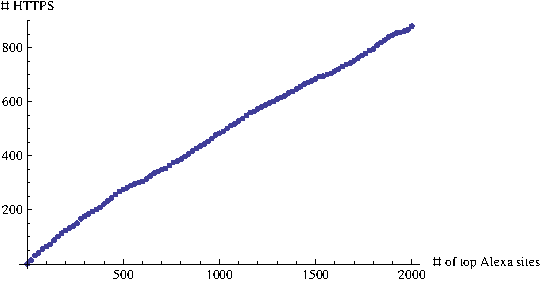
\includegraphics[width=70mm]{alexa_https.pdf}
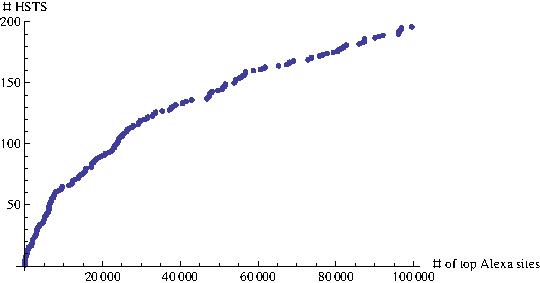
\includegraphics[width=70mm]{alexa_hsts.pdf}
\end{center}

\section{Common Deployment Patterns}

Most sites redirect straight to 

\subsection{Redirect straight to \s}

A plurality of sites redirect straight to a final destination of \s, where they serve an HSTS header. Of these:

\begin{itemize}
\item Only \todo{$1/4$} \iSD~in the header at \s~(thus protecting the original URL).
\item Roughly \todo{$1/2$} of the sites do not send an HSTS header over \s~and do not \iSD.
\item \todo{$1/4$} of the sites improperly send an HSTS header over plain HTTP%.
\end{itemize}

\subsection{Redirect straight to \sw}

\item Roughly \todo{$40\%$} of the sites \iSD~in the header at \sw.
\item Few sites send an HSTS header over \s.
\item \td{discuss separately?}{Roughly $40\%$ of the sites improperly send an HSTS header over plain HTTP.}

\subsection{Redirect to HTTPS}

\subsection{Redirect to \code{www}}

\section{Common Mistakes}
\todo{Or, as Buzzfeed would call it: 3 Ways Your "Secure" Site is Horribly Broken.}

\subsection{Permanently Insecure Redirects}

A common pattern is to redirect to \sw~when the user types \site{\genericsite} into their browser. The initial redirecting first page is necessarily insecure. If the site does not set an HSTS for \s, then this insecure redirect occuers \emph{every time} the user types \site{\genericsite} into their browser.

This is mitigated the browser cache retains an entry for \site{\genericsite}. However, it is undesirable to rely on the cache for such a critical security guarantee, and the protection does not apply for any other pages/resources on \h except the cached URL.

\subsection{Accidental HSTS Expiration}

It is possible to send an HSTS header at \h~along with a $30x$ redirect to $\sw$. However, browsers may cache $301$ aggressively by default. The browser will send \h visits directly to \sw, without visiting \s; thus, the browser will not see another HSTS header for \s, and it will slowly expire once the max-age is reached. If the max-age was set to a low value (e.g. for testing), the browser will also not see the updated value after the initial expiration.

Again, the security guarantee of HSTS is relegated to the presence of a cache entry.

\subsection{Clerical Mistakes}

$30\%$ of HSTS sites in our survey also send an HSTS header over \h or \hw. While an RFC-conforming browser is required to ignore this, RFC 6797\cite{rfc} also states that:

\begin{quotation}\it
An HSTS Host MUST NOT include the STS header field in HTTP responses conveyed over non-secure transport.
\end{quotation}

Sending the header over plain HTTP suggests an unfamiliarity with HSTS, \todo{apathy towards towards this specification}, or inadequate control over redirect configuration.

In our scans, we also encountered two occasional mistakes:

\begin{itemize}
\item Sending two HSTS headers in the same requests.
\item Using a comma instead of a semicolon to delimit the \iSD~directive.
\end{itemize}


\section{Issues with Improving HSTS Configuration}

\subsection{Implications of \iSD}
\label{includeSubDomains-issues}

In practice, using \iSD~may mot be straightforward at the top-level (\s) of an existing site because there is at least one subdomain that may break over HSTS. Possibilities for this include:

\begin{itemize}
\item Such a large change is usually accompanied by increasing the scope of secure redirects (``\emph{if} we're going to do it, we may as well do it all at once''), which may break certain clients that rely on plain HTTP.
\item \td{verify}{Insecure resources will fail to load and break pages that worked over HTTPS without HSTS (where they previously only caused a mixed-content warning).}
\item The server for a subdomain is not configured to use HTTPS.
\item It may be impractical/expensive/risky to furnish every subdomain server with a valid CA-signed certificate.
\item The browser will prevent the user from using self-signed certificates for any subdomains.
\item The browser will enforce HTTPS is for all subdomains even if there are other security measures in place (such as local testing or gating for a corporate network) that would otherwise allow the continued use of plain HTTP.
\end{itemize}

While it is desirable to address these issues and design any new domains with them in mind, any combination of known/uncertain issues with subdomains can hinder the adoption of HSTS with \iSD.

\subsection{Canonical Subdomain}

If the canonical domain for a site is \sw, the user may rarely load a page/resource from \s. This makes it more difficult to secure a fresh visit to \s, should the user ever visit it directly. It also  any other subdomains.

Currently, the simplest solution is to cause the browser to load a page/resource from \s; we discuss approaches below.


\section{Best Practice}


\subsection{Ideal Practice}


The strongest protection is to

\begin{itemize}
\item redirect every resource to HTTPS immediately
\end{itemize}

and serve well-formed  HSTS header:

\begin{itemize}
\item with every HTTPS request,
\item with a long \code{max-age} (at least $1$ year),
\item and with \iSD.
\end{itemize}

To be fully correct, the site must also:

\begin{itemize}
\item never send an HSTS header over plain HTTP.
\end{itemize}

This protects all future requests to the site or any of its subdomains. If the canonical site is \s, any requests to the site will automatically update the expiration date (including for subdomains).

Any security-conscious site should strive to deploy this full approach, if possible.

\subsection{Send an HSTS header whenever possible}

It is advisable to send an HSTS header on any request sent from a (sub)domain only intended to be accessed over HTTPS. In particular, the header should be sent from \s, \sw, and any subdomains. This ensures that HSTS is enabled on every subdomain as early as possible, without depending on other sub/superdomains.

In addition, every visit extends the expiration of HSTS.

\subsection{Send the most secure settings possible}

Every site should aim to ramp up its \code{max-age} as high as possible (at least to the popular default of $6$ or $12$ months).

As advocated in RFC 6797\td{cite section 14.4 specifically}{\cite{rfc}}, \code{includeSubdomains} should also be sent whenever possible. Although section \ref{includeSubDomains-issues} discusses issues with \iSD for \s, it is usually safe to send \iSD~on any particular subdomain, including \sw.

\subsection{Redirect Immediately and Securely}

Unless legacy use cases require plain HTTP support, every request should be redirected to HTTPS (using a $30x$ status) before any content is served.

Any redirect served over HTTPS should include an HSTS header, to ensure that the redirect is fully secured in the future.

A site should redirect to the HTTPS version of a URL before performing other canonicalization steps like adding/removing \code{www}. This ensures that HSTS will be applied to future redirects.

If all the redirect URLS and final destinations of a site are protected using \iSD~at the destination, a two-hop redirect and a separate HSTS setting for the redirect (sub)domain may seem redundant. However, the first redirect will be eliminated once HSTS in place, and continues to protect the redirect in case \iSD needs to be removed (e.g. to address issues similar to section \ref{includeSubDomains-issues}).

\subsection{Securing \s~from from a subdomain}

If most pages are served from a subdomain like \sw, securing the entire domain requires an additional step. A simple solution is to make a request to an uncached resource on \s, such as a $1$-pixel \code{<img>} tag (or an iframe) with a cache-busting parameter: \site{\s/img.jpg?[unique-value]}. It is not necessary to prevent this resource from redirecting, as long as it serves an HSTS header itself.

We have verified that the HSTS setting from the resource is recorded by Chrome. \todo{Firefox}

\section{Browser Considerations}

\subsection{HSTS Browser Support}

As of September 29, 2013, HSTS is currently supported in the desktop versions of Chrome, Firefox, and Opera. It is not supported in Internet Explorer or Safari.\cite{support}

In addition, the mobile versions of Chrome (iOS and Android) and Firefox (Android) support HSTS like their desktop counterparts\cite{mdn}.

\subsection{Chromium Preload List}

The Chromium project maintains a list of sites in one of its source files\td{cite}{sts-list}. A site can request to be included in this list with a combination of several requirements including:

\begin{itemize}
\item \code{force-https} - enables HTTPS for a site by default (without expiration).
\item \iSD - same as HSTS.
\item \code{pins} - specific pinned certificates.
\end{itemize}

Google Chrome and Chromium employ this list directly, enforcing the specified security measures.

Chrome considers HSTS to be part of the cache. The ``Empty the cache'' setting for clearing browsing data also wipes HSTS values.

\subsection{Opera}

Opera shares the WebKit-derived Blink engine with Chromium, so it exhibits the same HSTS behavior as Chrome.\footnote{Opera originally implemented support in Presto engine\cite{opera}, but Opera is closed-source, and \todo{does not provide explicit documentation about HSTS support since the transition. It behaves like Chrome for preload sites according to the network console.}}

\subsection{Firefox Preload List}

Firefox ``seeds'' its list by starting with the Chromium preload list, but performs additional filtering. A site is included in the Firefox preload list if:

\begin{itemize}
\item It is in the Chromium list.
\item It sends an HSTS header.
\item The \code{max-age} sent is at least $10886400$ ($18$ weeks).
\end{itemize}

\section{Conclusion}

\bibliographystyle{./IEEEtran}
\bibliography{hsts}

\end{document}
